%Correctness
\section{Correctness}

In this section we look at the correctness of the code generation process. Correctness can be described as the mapping shown in Figure \ref{fig:correctness_graph1}. 
Expressions in our system are compiled into the program code. 
Expressions can be evaluated by hand ($\delta$) to produce a value. 
Likewise the program can be executed to produce a final value. 
Correctness holds in the system if the value of the evaluation ($\delta$) is the 
same as a value achieved by execution.

\begin{figure}[htb]
    \centering
    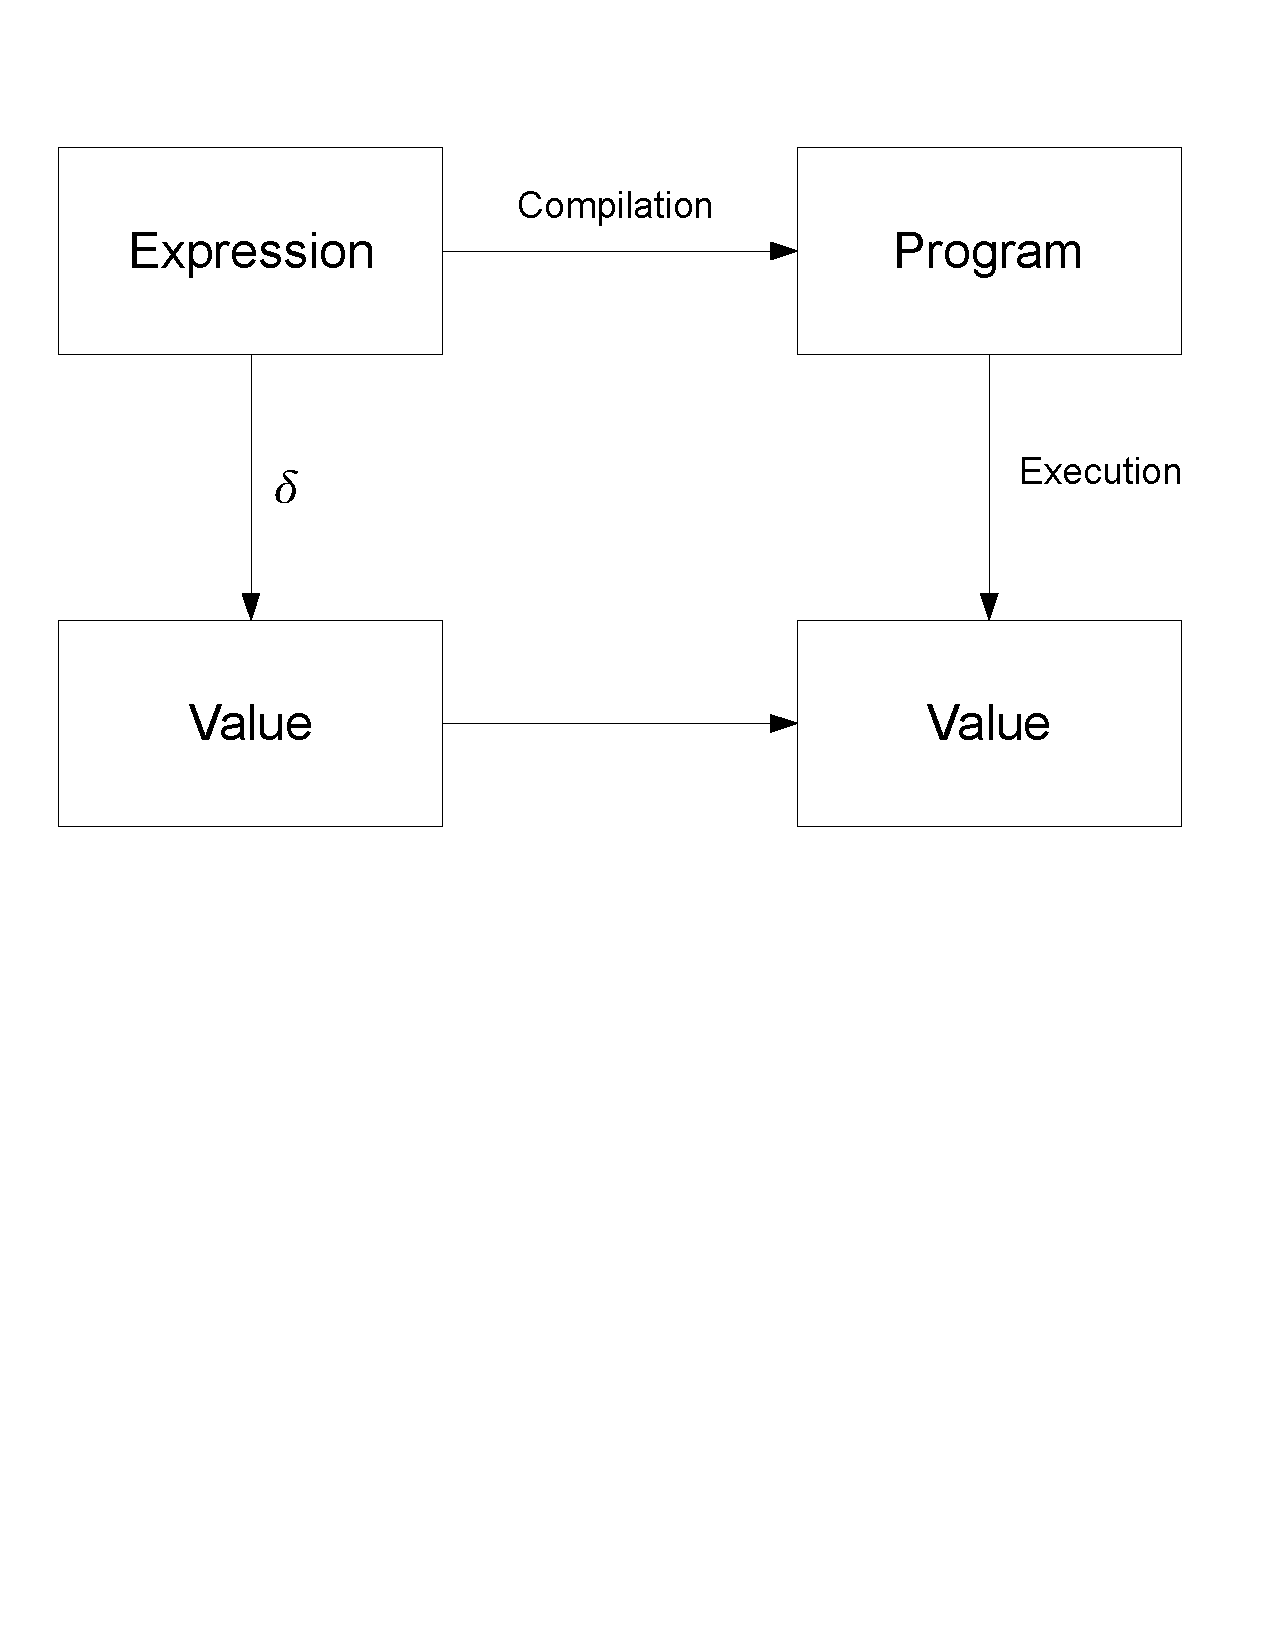
\includegraphics[trim= 10mm 120mm 10mm 10mm, clip, width=250px]{./images/correctness_graph1.pdf}
    \caption{Code Transformations}
    \label{fig:correctness_graph1}
\end{figure}

Our tool constructs executable code from the drawn diagram the constructs are 
defined in Sections \ref{sec:statechartsyn} and \ref{sec:statechartsem}. To justify 
the correctness we need 
to demonstrate the program structure generated from a graph structure is correct. 
To do so we extend Figure \ref{fig:correctness_graph1} to obtain 
Figure \ref{fig:correctness_graph2} to incorporate the transition construct. 
If each Figure \ref{fig:correctness_graph1} represents an individual block 
than the extended Figure \ref{fig:correctness_graph2} represents the several 
blocks with the ability to transition between them.

\begin{figure}[htb]
    \centering
    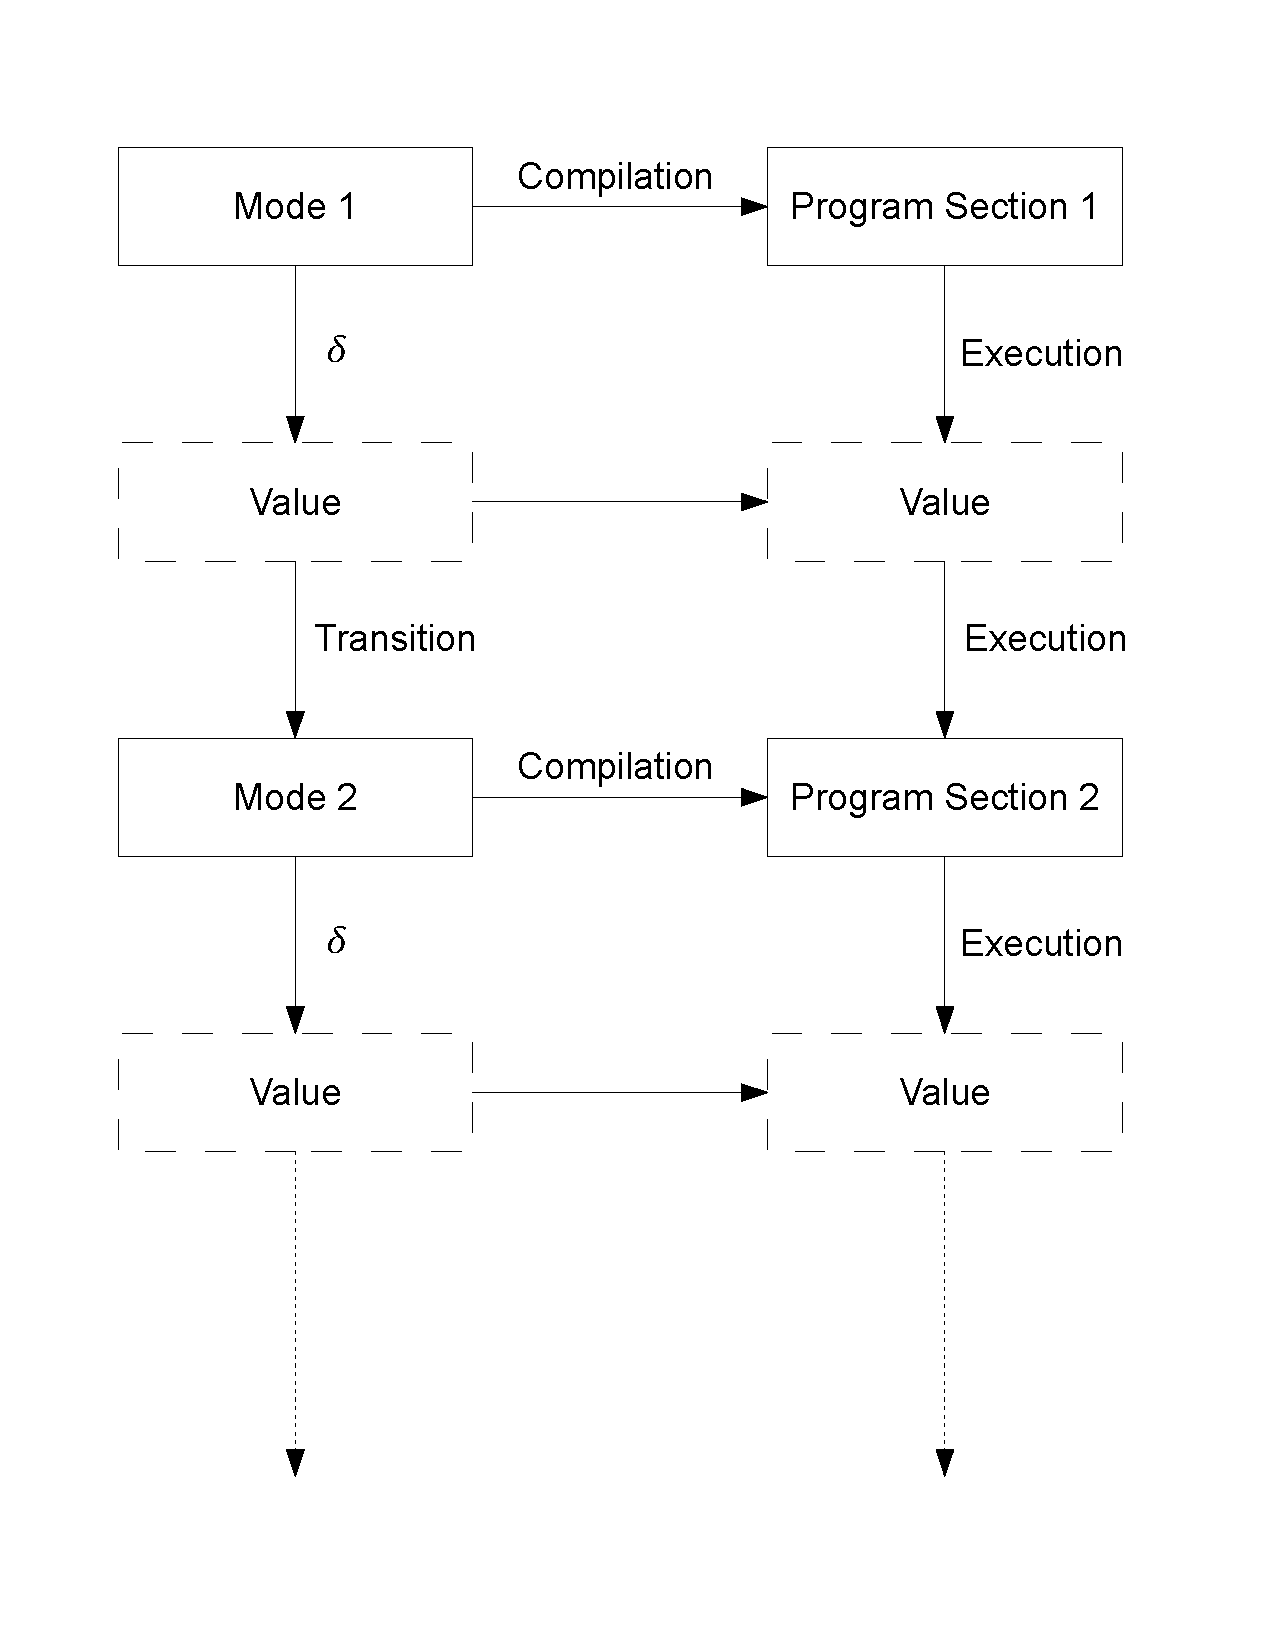
\includegraphics[trim= 10mm 30mm 10mm 10mm, clip, width=\imgmedium]{./images/correctness_graph2.pdf}
    \caption{Code Transition Structure}
    \label{fig:correctness_graph2}
\end{figure}

In this section we begin by showing that each of the transformations to code are 
correct by examining the basic atoms. We will start by looking at atoms that have the 
simplest assignments first.

\clearpage
\subsection{Atoms}

Each block in \plccharts compiles to their own atomic assign statements.
In the case were variables are used the type information is not present in 
the atomic assignment portion of the code generation. 
Variables are collected at compile time declared and initialized as part of 
the program construction. By collecting variables in this manner a variable 
with the same name but given two different types can be identified and will 
cause a compile error. Also the syntax of \plccharts uses ``:='' as an 
assign symbol, the final generated code will use the ``='' symbol.


\subsubsection{Start Block}

\begin{figure}[h]
	\centering
	
\includegraphics[width=\imgmedphoto]{./images/correctness_atom_start.png}
	\caption{Start Atom}
	\label{fig:correctness_atom_start}
\end{figure}

\begin{lstlisting}[frame=single]
(No atomic assignments or operations in code)
\end{lstlisting}

The start atom is the only atom in our system that does not generate any actual 
code for the atom itself. Instead the start atom is used as a place holder so that 
transitions can be constructed. It also structurally indicates where the program 
should start. Since the start block contains no atomic code it is trivially correct 
as it does nothing itself.


\subsubsection{Delay Block}

\begin{figure}[h]
	\centering
	
\includegraphics[width=\imgmedphoto]{./images/correctness_atom_delay.png}
	\caption{Delay Atom}
	\label{fig:correctness_atom_delay}
\end{figure}

\begin{lstlisting}[frame=single]
delayms(10);
\end{lstlisting}

The delay atom generates ``delayms($<$Expression$>$)''. The expression is mirrored
in the diagram. The units shown in Figure \ref{fig:correctness_atom_delay} as ``ms'' 
are omitted in the code. The units in the visual representation serves as a reminder to the user 
that the delay is always measured in milliseconds. Expressions follow the syntax 
given in Section \ref{sec:statechartsyn}. Since there are no assignments to values,
the mappin gfrom evaluated values (none) to executed values (none) is trivially correct.


\subsubsection{Output Block}

\begin{figure}[h]
	\centering
	
\includegraphics[width=\imgmedphoto]{./images/correctness_atom_output.png}
	\caption{Output Atom}
	\label{fig:correctness_atom_output}
\end{figure}

\begin{lstlisting}[frame=single]
PORTOUT = 0xF2;
\end{lstlisting}

The output atom generated refers to PORTOUT, which is mapped on a hardware level 
to the PLC hardware's output port. This is done to allow the hardware manufacturer 
a bit of flexability. In our implementation PORTOUT can be assigned any 8-bit value. 
Any values larger than 8-bit will be trucated. 
In the example shown in Figure \ref{fig:correctness_atom_output} we can see that the 
assignment in the diagram is ``PORTOUT := 0xF2''. We can say that the meaning of 
this line is $\delta(PORTOUT) = (F2)_{16}$. The final compiled output code is 
``PORTOUT = 0xF2''. We can see that $Execution(PORTOUT) = (F2)_{16}$ since we 
have a direct mapping from the value in diagram to value in 
execution ($\delta(PORTOUT) = Execution(PORTOUT)$), we can conclude that 
the assignment in the output block is done correctly with respect to the diagram.

\clearpage
\subsubsection{Input Block}

\begin{figure}[h]
	\centering
	
\includegraphics[width=\imgmedphoto]{./images/correctness_atom_input.png}
	\caption{Input Atom}
	\label{fig:correctness_atom_input}
\end{figure}

\begin{lstlisting}[frame=single]
var = PORTIN;
\end{lstlisting}


We can see in Figure \ref{fig:correctness_atom_input} that the diagram clearly shows
the assignment ``int var := PORTIN''. We can say the meaning of the assignment in 
the diagram is $\delta(var) = PORTIN$. The final compiled code for the atom is 
``var = PORTIN''. The left hand side must be a valid variable name as specified 
in the syntax of \plccharts (see section \ref{sec:statechartsyn}). 
The variable can be any type however PORTIN will always be read as an 8-bit integer. 
Any variable on the left hand side that is not integer would have PORTIN 
automatically casted to the appropriate type. Thus we can see that 
$Execution(var) = PORTIN$. We note that there is a direct mapping from diagram
$value$ to execution $value$, that is: $\delta(var) = Execution(var) = PORTIN$. 
Thus by our definition of correctness as defined in the beginning of this 
section and Figure \ref{fig:correctness_graph1}, we can conclude that 
the input block is correct.


\subsubsection{Store Block}

\begin{figure}[h]
	\centering
	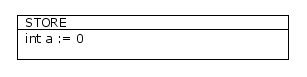
\includegraphics[width=\imgmedphoto]{./images/correctness_atom_store_single.png}
	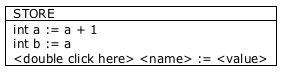
\includegraphics[width=\imgmedphoto]{./images/correctness_atom_store.png}
	\caption{Store Atom}
	\label{fig:correctness_atom_store}
\end{figure}

Single Assign (Left Diagram)
\begin{lstlisting}[frame=single]
a = 0;
\end{lstlisting}

Multiple Assign (Right Diagram)
\begin{lstlisting}[frame=single]
a = a + 1;
b = a;
\end{lstlisting}

The \emphasize{Store Block} is used for assignments. In the left diagram of 
Figure \ref{fig:correctness_atom_store} we see a \emphasize{Store Block} with one 
assign statement and in the right diagram of Figure \ref{fig:correctness_atom_store} we see 
that store blocks can also contain multiple atomic assign statements. 

Looking at the left diagram first, we note that the assign statement is ``int a := 0'' 
that is to mean $\delta(a) = 0$. We see the final generated code is ``$a = 0$'' 
meaning $Execution(a) = 0$. We see that $\delta(a) = Execution(a)$ that is to 
say there exists a mapping from the value in the diagram to the value from the execution. 
We can say that the code generated is correct with respect to the diagram. 
Looking at the right diagram we see that each line of the \emphasize{Store Block} 
becomes own atomic assign statement in the code. We see that the diagram 
has ``int a := a +1'' and ``int b := a'' with evaluations $\delta(a) = a + 1, \delta(b) = a$. 
The generated code is then ``a = a + 1'' and ``b = a'' with the executed values 
$Execution(a) = a + 1, Execution(b) = a$. We can see at this point that $\delta(a) = Execution(a)$ 
and $\delta(b) = Execution(b)$. Thus we can conclude that the \emphasize{Store Block} 
generated code is correct with respect to our diagram. We note that we can create equivalent 
diagrams by having two single line store atoms. 
Thus, it is not difficult to see that the right diagram is just a visual simplification one dual 
line \emphasize{Store Block}, corresponds to several atomic assigns. Being able to group 
assigns together into one atomic diagram removes the need to have several atomic assign blocks.
This is ultimately removes visual clutter and makes the overall diagram simpler.


\subsection{Constructors and Transitions}

Constructors takes the atoms and places structural elements around them. 
In the example code below we demonstrate the constructed sections for any arbitrary 
compiled code. On lines 00-07 we have the variable initialization section, 
any variables used are initialized and the type is declared here.
Variables in our program are collected at compile time by scanning all the diagram 
objects and collecting any variables used. Any conflicts where a variable is given inconsistent types
are caught and will cause a code generation error. The initialization section will 
set all variables to a default value after defning the type.

The generated constructs also exist to provide a way for each of the states to terminate the program
if no departing transitions exist. This is accomplished by lines 32-33 an ``end of file'' label 
is generated to mark the end of the program followed by a return statement to end the 
program and return control to the programmable logic controller chip. On recieving a 
return the \emphasize{Programmable Logic Controller} will hold all last known values 
on every port and halt, this simulates a stop.


\begin{lstlisting}[frame=single]
00 // BEGIN VARIABLE INITIALIZATIONS //
01 int a = 0;
02 int b = 0;
03 float c = 0;
05 double d = 0;
06 byte e = 0;
07 // END VARIABLE INITIALIZATIONS //
...
32 EOF:
33 return;
\end{lstlisting}

Transitions are used to string together a sequence of atoms in order to perform the computations necessary in our program. In order to show correctness we must show that the transitions are structurally correct. We must show transitions will correctly map modes in the right sequence. Figure \ref{fig:correctness_graph2} shows how transitions factor into our correctness justification. Figure \ref{fig:correctness_graph2} states that in addition to our original correctness justification we must also demonstrate that the transitions take us to the same modes and program sections.

\clearpage
\begin{figure}[htp]
	\centering
	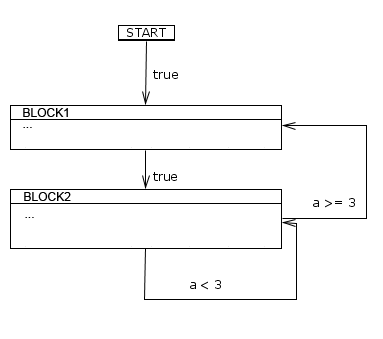
\includegraphics[width=\imgmedphoto]{./images/correctness_ex_transition.png}
	\caption{Transitions}
	\label{fig:correctness_ex_transition}
\end{figure}

%\begin{minipage}{\textwidth}
\begin{lstlisting}[frame=single]
00 // BEGIN VARIABLE INITIALIZATIONS //
01 ...
03 // END VARIABLE INITIALIZATIONS //
04
05 BLUID0:
06 //////////////////////////////////////
07 //        PROGRAM START             //
08 //////////////////////////////////////
09 goto BLUID1;
10 goto EOF;
11
12 BLUID1:
13 //////////////////////////////////////
14 //        BLOCK1                    //
15 //////////////////////////////////////
16 ...
17 
18 goto BLUID2;
19 goto EOF;
20
21 BLUID2:
22 //////////////////////////////////////
23 //        BLOCK2                    //
24 //////////////////////////////////////
25 ...
26
27 if (a >= 3) goto BLUID1;
28 if (a < 3) goto BLUID2;
39 goto EOF;
30
31 EOF:
32 return;
\end{lstlisting}
%\end{minipage}

Starting by looking at the code above we can see that our first entry point into the program is the ``PROGRAM START'' block. This refers to the \emphasize{Start Block} in our diagram. During compilation the entire diagram is scanned to ensure there is one and only one start block. The generated code for the start block is then placed at the top of the program to ensure it is the first entry point of the program after initializers. 

Transitions in our program are compiled to ``goto'' statements. Each block is given a unique ``Block Unique Identifier'' which is a line label starting with ``BLUID''. BLUID's are generated as each block is scanned at compile time and a monotonically increasing number is appended to the end of the label. The ``goto'' transitions are insertedr after the atomic block assignments have been made.

Looking at the diagram given in Figure \ref{fig:correctness_ex_transition} we note that the \emphasize{Start Block} transitions to ``BLOCK1'' with an edge guarded by ``true''. In the code ``BLOCK1'' has label ``BLUID1'' associated with its section of code. We see that the generated code for the \emphasize{Start Block} has a ``goto BLUID1'' on line 9. This corresponds to transition leaving the \emphasize{Start Block}. Next we have a transition from ``BLOCK1'' to ``BLOCK2'' in Figure \ref{fig:correctness_ex_transition}. We can see the code corresponding to the transition on line 18 ``goto BUILD2'' where ``BLUID2'' refers to ``BLOCK2''. Finally we note the two guarded transitions leaving ``BLOCK2''. For the guarded edge ``$a >= 3$'' we can see the generated code ``\texttt{if (a >= 3) goto BLUID1}'' on line 27. We note that ``BLUID1'' refers to ``BLOCK1'' in the diagram so the transition goes from ``BLOCK2'' to ``BLOCK1'' which is correct. For the transition guarded by ``$a < 3$'' we note the generated code on line 28 ``\texttt{if (a < 3) goto BLUID2}''. We see that ``BLUID2'' refers to ``BLOCK2'' so the transition is a self loop, which is correct with respect to the diagram in Figure \ref{fig:correctness_ex_transition}. Since all the transitions are generated correctly for any arbitrary block we can conlude that the transtions are structurally correct in our system.


\clearpage
\subsection{Correctness of Translation}

\subsubsection{Table Representation}

In order to show the correctness of the execution it is necessary to identify the differences 
between graphical evaluation and execution. Both contain a ``mode'' in execution the 
mode is directly associated to a set of line numbers. Line numbers are not in the diagram view. 
Both have variables and modes, and correct execution can be defined as a trace where all 
modes and variables are identical. We will use tables to compare the diagram trace vs the execution.
We will start with a simple start diagram as shown in Figure \ref{fig:correctness_ex_start}.
A diagram trace is shown in Table \ref{table:BasicDiagOnly}. 

\begin{figure}[h]
	\centering
	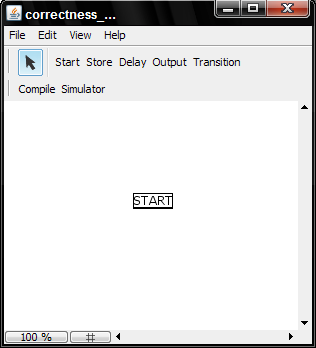
\includegraphics[width=\imgsmall]{./images/correctness_ex_start.png}
	\caption{Singular Start Block}
	\label{fig:correctness_ex_start}
\end{figure}


The accompanying generated \emphasize{IL} code for Figure \ref{fig:correctness_ex_start}.

\begin{lstlisting}[frame=single]
00 // BEGIN VARIABLE INITIALIZATIONS //
01 // END VARIABLE INITIALIZATIONS //
02
03 BLUID0:
04 //////////////////////////////////////
05 //        PROGRAM START             //
06 //////////////////////////////////////
07 goto EOF;
08 
09 EOF:
10 return;
\end{lstlisting}

\begin{table}[htcb]
	\caption{Start Diagram shown in Figure \ref{fig:correctness_ex_start}}
	\centering
		\begin{tabular}{| l | l | l | l |}
			\hline
			\textbf{Mode} & \textbf{Variables} & \textbf{Transitions} & \textbf{Next Mode} \\
			\hline
			start & (none) & (none) & (none meaning stop) \\
			\hline
			(none) & (none) & (none) & (none) \\
			\hline
		\end{tabular}
	\label{table:BasicDiagOnly}
\end{table}

To show an execution trace we replace mode with line number and we get the following Table \ref{table:BasicExecOnly}.

\begin{table}[htcb]
	\caption{Start code execution for compiled code from Figure \ref{fig:correctness_ex_start}}
	\centering
		\begin{tabular}{| l | l | l | l |}
			\hline
			\textbf{Line} & \textbf{Variables} & \text{Code} & \textbf{Next Executed Line} \\
			\hline
			00 & (none) & (comment) & 07 \\
			\hline
			07 & (none) & \texttt{goto EOF} & 09 \\
			\hline
			09 & (none) & (line label) & 10 \\
			\hline
			10 & (none) & return & (stop) \\
			\hline
		\end{tabular}
	\label{table:BasicExecOnly}
\end{table}

It is not to difficult to see that from lines 00 to 07 we are in the ``start'' mode so we can append a
mode marker to the end of the table. We can also identify that line 09 ``EOF'' represents the end of the
file and thus has no mode associated with it.

\begin{table}[htcb]
	\caption{Start code execution for compiled code from Figure \ref{fig:correctness_ex_start} extended}
	\centering
		\begin{tabular}{| l | l | l | l | l |}
			\hline
			\textbf{Line} & \textbf{Variables} & \textbf{Code} & \textbf{Next Executed Line} & \textbf{Mode}\\
			\hline
			00 & (none) & (comment) & 07 & \textbf{start} \\
			\hline
			07 & (none) & \texttt{goto EOF} & 09 &  \textbf{start}\\
			\hline
			09 & (none) & (line label) & 10 & \textbf{none} \\
			\hline
			10 & (none) & return & (stop) & \textbf{none} \\
			\hline
		\end{tabular}
	\label{table:BasicExecMode}
\end{table}

We can already see that the trace and execution will produce the same outcome
if we compare the two tables. For ease of comparison we can
merge the two tables side by side so we can directly compare each executed 
line to its associated graph.

\begin{table}[htcb]
	\caption{Start code execution combined table. For Figure \ref{fig:correctness_ex_start}}
	\centering
	\tablefontsize
		\begin{tabular}{| p{0.06\textwidth} | p{0.1\textwidth} | p{0.15\textwidth} | p{0.06\textwidth} | p{0.05\textwidth} | p{0.1\textwidth} | p{0.2\textwidth} | p{0.07\textwidth} |}
			\hline
			\textbf{Mode} 		&	\textbf{Var (Diag)} 		& 	\textbf{Transitions} 		& 	\textbf{Next}		&	\textbf{Line}		&	\textbf{Var (Exec)	}	&	\textbf{Code}	&	\textbf{Next LN} \\
			\hline
			start 				&	(none)						&	(none)						&	(none meaning stop)	&	00					&	(none)					& 	(comment)		&	07 \\
			\hline
								&								&								&						&	07					& 	(none)					& 	goto EOF		& 	10 \\
			\hline
								&								&								&						&	10					&	(none)					&	return			&	(stop) \\
			\hline
		\end{tabular}
	\label{table:BasicExecCombined}
\end{table}

In Table \ref{table:BasicExecCombined} we can easily 
compare the execution vs the diagram trace. 
We can see that line numbers can be associated with 
a mode despite not having one themselves. 
In order to verify correct execution it is necessary to 
show that the sequence of modes and values are the same. 
In the above example in which we run our first trivially 
simple start code snippet it is easy to see that this holds. 
Therefore we can conclude that the execution is 
correct for the start diagram shown in Figure \ref{fig:correctness_ex_start}.

\subsubsection{Start Diagram Execution}

The start diagram analysis was already done as a previous example to 
construct our comparision tables please see Table \ref{table:BasicExecCombined}. 
We may note that the only mode is ``start'' and that the mode is the same 
through the executed line by line trace. We can also note that the code stops after ``start'' 
mode is finished which also is correct behaviour. 
Finally there are no variables listed in
our system so variables are trivially correct.

\subsubsection{Delay Diagram Execution}

\begin{figure}[h]
	\centering
	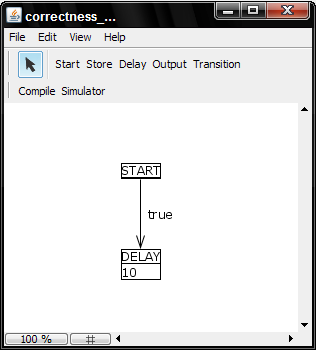
\includegraphics[width=\imgmedsmall]{./images/correctness_ex_delay.png}
	\caption{Delay Block}
	\label{fig:correctness_ex_delay}
\end{figure}

Generated \emphasize{IL} code for diagram in Figure \ref{fig:correctness_ex_delay}.
\begin{lstlisting}[frame=single]
00 // BEGIN VARIABLE INITIALIZATIONS //
01 // END VARIABLE INITIALIZATIONS //
02 
03 BLUID0:
04 //////////////////////////////////////
05 //        PROGRAM START             //
06 //////////////////////////////////////
07 goto BLUID1;
08 goto EOF;
09 
10 BLUID1:
11 //////////////////////////////////////
12 //        DELAY                     //
13 //////////////////////////////////////
14 delayms(10);
15 goto EOF;
16
17 EOF:
18 return;
\end{lstlisting}


\begin{table}[h]
	\caption{Delay code execution combined table. For Figure \ref{fig:correctness_ex_delay}}
	\centering
	\tablefontsize
		\begin{tabular}{| p{0.06\textwidth} | p{0.1\textwidth} | p{0.15\textwidth} | p{0.06\textwidth} | p{0.05\textwidth} | p{0.1\textwidth} | p{0.2\textwidth} | p{0.07\textwidth} |}
			\hline
			\textbf{Mode} 		&	\textbf{Var (Diag)} 		& 	\textbf{Transitions} 		& 	\textbf{Next}		&	\textbf{Line}		&	\textbf{Var (Exec)	}	&	\textbf{Code}	&	\textbf{Next LN} \\
			\hline
			start 				&	(none)						&	if (true) delay				&	delay				&	00					&	(none)					& 	(comment)		&	07 \\
			\hline
								&								&								&						&	07					& 	(none)					& 	goto BLUID1		& 	10 \\
			\hline
			delay				&	(none)						&	(none)						&	(stop)				&	10					&	(none)					&	(line label)	&	14 \\
			\hline
								&								&								&						&	14					&	(none)					&	delayms(10)		&	15 \\
			\hline
								&								&								&						&	15					&	(none)					&	goto EOF		&	17 \\
			\hline
								&								&								&						&	17					&	(none)					&	(line label)	&	18 \\
			\hline
								&								&								&						&	17					&	(none)					&	return			&	(stop) \\
			\hline
		\end{tabular}
	\label{table:DelayExecCombined}
\end{table}

Once again in this example we don't have any variables so they 
are easily verified by checking that in both cases there are no variables. 
All that's left to justify correctness is ensuring the sequence of modes 
is executed correctly. It should be easy to see that the sequence: 
start, delay, stop. Is clearly implemented by the executed code from the 
Table \ref{table:DelayExecCombined}. We can therefore conclude that the 
executed code trace is correct with respect to the original diagram.

\subsubsection{Output Diagram Execution}

\begin{figure}[htb]
	\centering
	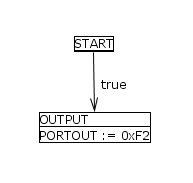
\includegraphics[width=\imgmedsmall]{./images/correctness_ex_output.png}
	\caption{Output Block}
	\label{fig:correctness_ex_output}
\end{figure}

Generated \emphasize{IL} code for diagram in Figure \ref{fig:correctness_ex_output}.
\begin{lstlisting}[frame=single]
00 // BEGIN VARIABLE INITIALIZATIONS //
01 // END VARIABLE INITIALIZATIONS //
02 
03 BLUID0:
04 //////////////////////////////////////
05 //        PROGRAM START             //
06 //////////////////////////////////////
07 goto BLUID1;
08 goto EOF;
09 
10 BLUID1:
11 //////////////////////////////////////
12 //        OUTPUT                    //
13 //////////////////////////////////////
14 PORTOUT = 0xF2;
15 goto EOF;
16 
17 EOF:
18 return;
\end{lstlisting}

\begin{table}[htcb]
	\caption{Output code execution combined table. For Figure \ref{fig:correctness_ex_output}}
	\centering
	\tablefontsize
		\begin{tabular}{| p{0.05\textwidth} | p{0.1\textwidth} | p{0.14\textwidth} | p{0.05\textwidth} | p{0.05\textwidth} | p{0.12\textwidth} | p{0.2\textwidth} | p{0.07\textwidth} |}
			\hline
			\textbf{Mode} 		&	\textbf{Var (Diag)} 		& 	\textbf{Transitions} 		& 	\textbf{Next}		&	\textbf{Line}		&	\textbf{Var (Exec)	}	&	\textbf{Code}	&	\textbf{Next LN} \\
			\hline
			start 				&	PORTOUT = 0					&	if (true) output			&	output				&	00					&	PORTOUT = 0				& 	(comment)		&	07 \\
			\hline
								&								&								&						&	07					&   PORTOUT = (no change)	&	goto BLUID		&	10 \\
			\hline
			output				&	PORTOUT = 0xF2				&	(none)						&	(stop)				&	10					&	PORTOUT = (no change)	&	(line label)	&	14 \\
			\hline
								&								&								&						&	14					&	PORTOUT = 0xF2			&	PORTOUT = 0xF2	&	15 \\
			\hline
								&								&								&						&	15					&	PORTOUT = (no change)	&	goto EOF		&	17 \\
			\hline
								&								&								&						&	17					&	PORTOUT = (no change)	&	(line label)	&	18 \\
			\hline
								&								&								&						&	18					&	PORTOUT = (no change)	&	return			&	(stop) \\
			\hline
		\end{tabular}
	\label{table:OutputExecCombined}
\end{table}

First we make a note that PORTOUT is an special variable that is 
used to send an output to the ports on the device.
According to the hardware specification section PORTOUT is initialized 
to 0 when the device first starts up. Likewise PORTOUT is zero until 
changed in our diagram. Understanding this the rest of the code trace 
is as follows: \{(start, PORTOUT = 0), (output, PORTOUT = 0xF2)\} where
we observe that our tuple comprises of (mode, variables). 
It is not difficult to see that our two code traces produce this
sequence and by our definition we can conclude that our
output execution is correct with respect to the diagram.


\subsubsection{Input Diagram Execution}

\begin{figure}[h]
	\centering
	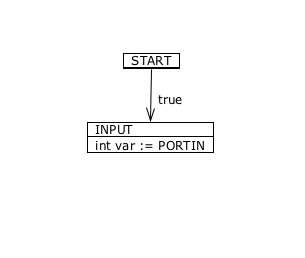
\includegraphics[width=\imgmedsmall]{./images/correctness_ex_input.png}
	\caption{Input Block}
	\label{fig:correctness_ex_input}
\end{figure}

Generated \emphasize{IL} code for the diagram in Figure \ref{fig:correctness_ex_input}.
\begin{lstlisting}[frame=single]
00 // BEGIN VARIABLE INITIALIZATIONS //
01 int var = 0;
02 // END VARIABLE INITIALIZATIONS //
03 
04 BLUID0:
05 //////////////////////////////////////
06 //        PROGRAM START             //
07 //////////////////////////////////////
08 goto BLUID1;
09 goto EOF;
10
11 BLUID1:
12 //////////////////////////////////////
13 //        Input                    //
14 //////////////////////////////////////
15 var = PORTIN;
16 goto EOF;
17
18 EOF:
19 return;
\end{lstlisting}

\begin{table}[htcb]
	\caption{Input code execution combined table. For Figure \ref{fig:correctness_ex_input}}
	\centering
	\tablefontsize
		\begin{tabular}{| p{0.05\textwidth} | p{0.1\textwidth} | p{0.14\textwidth} | p{0.05\textwidth} | p{0.05\textwidth} | p{0.12\textwidth} | p{0.2\textwidth} | p{0.07\textwidth} |}
			\hline
			\textbf{Mode} 		&	\textbf{Var (Diag)} 		& 	\textbf{Transitions} 		& 	\textbf{Next}		&	\textbf{Line}		&	\textbf{Var (Exec)	}	&	\textbf{Code}	&	\textbf{Next LN} \\
			\hline			
								&								&								&						&	00					& 	var = UNDEFINED			&	(comment)		&	01	\\
			\hline
								&								&								&						&	01					&	var = 0					&	int var = 0		&	04	\\
			\hline
			start 				&	var = 0						&if (true) $\rightarrow$ input	&	input				&	04					&	var = (no change)		& 	(comment)		&	08	\\
			\hline
								&								&								&						&	08					&	var = (no change)		&	goto BLUID1		&	11	\\
			\hline
			input				&	var = PORTIN				&	(none)						&	(stop)				&	11					&	var = (no change)		&	(line label)	&	15	\\
			\hline
								&								&								&						&	15					&	var = PORTIN			&	var = PORTIN	&	16	\\
			\hline
								&								&								&						&	16					&	var = (no change)		&	goto EOF		&	18	\\
			\hline
								&								&								&						&	18					&	var = (no change)		&	(line label)	&	19	\\
			\hline
								&								&								&						&	19					&	var = (no change)		&	return			&	(stop)	\\
			\hline
		\end{tabular}
	\label{table:InputExecCombined}
\end{table}

We must first note in this code trace that inputs require a variable in order to store
their data. These inputs are initialized at the beginning of the execution. 
Initialization is not required for our diagram it is understood that an initial
value of 0 is used. Our table starts with line 00, and 01 which initialize 
our variable, we consider this ``house keeping'' and on the left side of our table we
do not associate this process with one of our diagram modes. This time the start
mode occurs 3 rows down with the corresponding line 04. The execution of the start block 
and diagram is identical to previous examples with the exception of different line numbers.
The sequence of modes and variables is observed as {(start, var = 0), (input, var = PORTIN)}.
We can observed that ``var'' is set to ``PORTIN'' on row 5 in the diagram. Tn the 
execution the corresponding set occurs on row 6. We note the sequence of modes and variables are identical.
Thus according to our definition of correctness we have shown that both diagram
and execution follow the same modes and variable values in the same sequence. 
We can conclude from this that the execution of the input code is correct
with respect to the diagram.

\subsubsection{Store Diagram Execution}

\begin{figure}[h]
	\centering
	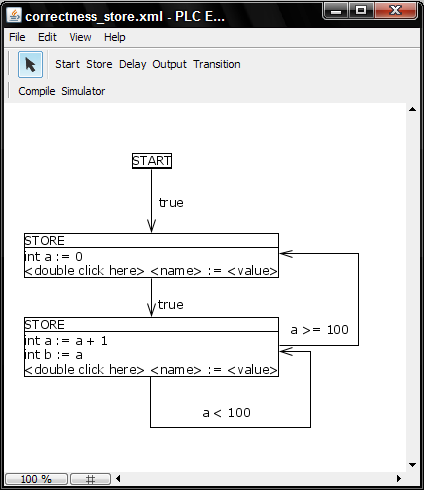
\includegraphics[width=\imgmedphoto]{./images/correctness_ex_store.png}
	\caption{Store Block Example}
	\label{fig:correctness_ex_store}
\end{figure}


Generated \emphasize{IL} code for diagram in Figure \ref{fig:correctness_ex_store}.
\begin{lstlisting}[frame=single]
00 // BEGIN VARIABLE INITIALIZATIONS //
01 int a = 0;
02 int b = 0;
03 // END VARIABLE INITIALIZATIONS //
04
05 BLUID0:
06 //////////////////////////////////////
07 //        PROGRAM START             //
08 //////////////////////////////////////
09 goto BLUID1;
10 goto EOF;
11
12 BLUID1:
13 //////////////////////////////////////
14 //        STORE                     //
15 //////////////////////////////////////
16 a = 0;
17 
18 goto BLUID2;
19 goto EOF;
20
21 BLUID2:
22 //////////////////////////////////////
23 //        STORE                     //
24 //////////////////////////////////////
25 a = a + 1;
26 b = a;
27
28 if (a >= 3) goto BLUID1;
29 if (a < 3) goto BLUID2;
30 goto EOF;
31
32 EOF:
33 return;
\end{lstlisting}


\begin{table}[htcb]
	\caption{Store code execution combined table. For Figure \ref{fig:correctness_ex_store}}
	\centering
	\tablefontsize
		\begin{tabular}{|p{0.01\textwidth} | p{0.05\textwidth} | p{0.1\textwidth} | p{0.14\textwidth} | p{0.05\textwidth} | p{0.05\textwidth} | p{0.12\textwidth} | p{0.2\textwidth} | p{0.07\textwidth} |}
			\hline
			\textbf{\#} & \textbf{Mode} 		&	\textbf{Var (Diag)} 		& 	\textbf{Transitions} 		& 	\textbf{Next}		&	\textbf{Line}		&	\textbf{Var (Exec)	}	&	\textbf{Code}	&	\textbf{Next LN} \\
			\hline			
			1&					&								&								&						&	00					& 	a = UNDEFINED \newline	b = UNDEFINED	&	(comment)		&	01	\\
			\hline
			2&					&								&								&						&	01					&	a = 0 \newline b = UNDEFINED	&	int a = 0				&	02	\\
			\hline
			3&					&								&								&						&	02					&	a = 0 \newline b = 0		&	int b = 0					& 	09	\\
			\hline
			4&start				&	a = 0 \newline b = 0		&	if (true) $\rightarrow store_1$	& $store_1$			&	09					&	a = $NC$ \newline b = $NC$	&	goto BLUID1					&	12	\\
			\hline
			5&$store_1$			&	a = 0 \newline b = $NC$		&	if (true) $\rightarrow store_2$ & $store_2$			&	12					&	a = $NC$ \newline b = $NC$	&	(line label)				&	16	\\
			\hline
			6&					&								&								&						&	16					&	a = 0 \newline b = $NC$		&	a = 0						&	18	\\
			\hline
			7&					&								&								&						&	18					&	a = $NC$ \newline b = $NC$	&	goto BLUID2					&	21	\\
			\hline	
			8&$store_2$			&	a = 1	\newline b = 1		&	if ($a \geq 3$) $\rightarrow store_1$ \newline
																	if ($a < 3$) $\rightarrow store_2$ &	$store_2$	&	21					&	a = $NC$ \newline b = $NC$	&	(line label)				&	25	\\
			\hline
			9&					&								&								&						&	25					&	a = 1 \newline b = $NC$		&		a = a + 1				&	26	\\
			\hline
			10&					&								&								&						&	26					&	a = $NC$ \newline b = 1		&		b = a					&	28	\\
			\hline
			11&					&								&								&						&	28					&	a = $NC$ \newline b = $NC$	& if (a \textgreater= 3) goto BLUID1 		&	29	\\
			\hline
			12&					&								&								&						&	29					&	a = $NC$ \newline b = $NC$	& if (a \textless 3) goto BLUID2		&	18	\\
			\hline
			13&$store_2$			&	a = 2	\newline b = 2		&	if ($a \geq 3$) $\rightarrow store_1$ \newline
																	if ($a < 3$) $\rightarrow store_2$ &	$store_2$	&	21					&	a = $NC$ \newline b = $NC$	&	(line label)				&	25	\\
			\hline
			14&					&								&								&						&	25					&	a = 2	\newline b = $NC$	&	a = a + 1					&	26	\\
			\hline
			15&					&								&								&						&	26					&	a = $NC$ \newline b = 2		&	b = a						&	28	\\
			\hline
			16&					&								&								&						&	28					&	a = $NC$ \newline b = $NC$	& if (a \textgreater= 3) goto BLUID1		&	29	\\
			\hline
			17&					&								&								&						&	29					&	a = $NC$ \newline b = $NC$	& if (a \textless 3) goto BLUID2		&	21	\\
			\hline
			18&$store_2$			&	a = 3	\newline b = 3		&	if ($a \geq 3$) $\rightarrow store_1$ \newline
																	if ($a < 3$) $\rightarrow store_2$ &	$store_1$	&	21					&	a = $NC$ \newline b = $NC$	&	(line label)				&	25	\\
			\hline
			19&					&								&								&						&	25					&	a = 3	\newline b = $NC$	&	a = a + 1					&	26	\\
			\hline
			20&					&								&								&						&	26					&	a = $NC$ \newline b = 3		&	b = a						&	28	\\
			\hline
			21&					&								&								&						&	28					&	a = $NC$ \newline b = $NC$	& if (a \textgreater= 3) goto BLUID1		&	12	\\
			\hline
			22&$store_1$			&	a = 0 \newline b = $NC$		&	if (true) $\rightarrow store_2$ & $store_2$			&	12					&	a = $NC$ \newline b = $NC$	&	(line label)				&	16	\\
			\hline
			23&\multicolumn{8}{|c|}{...}\\
			\hline
		\end{tabular}
	\label{table:StoreExecCombined}
\end{table}

The reader should note that we have shortened ``no change'' in the previous tables to ``NC'' in order to fit
it in the tables.  Similar to the input example the store example also has variables that must be initialized 
before it can enter it's first state. Lines 00-02 in the Table \ref{table:StoreExecCombined} represent the 
``house keeping'' steps required in order to define, setup and initialize the variables. The entry of the start
mode represents the start of our diagram. The reader can see from Table \ref{table:StoreExecCombined} the two
variables are considered initialized to 0 in the diagram, that is ``a = 0, b = 0''. We may also note that this
is taken care in the execution by lines 01 and 02.

On line 12 we enter our first store block which we
have denoted $store_1$. Observe that only variable ``a'' is modified in this store block thus ``b'' takes on 
a value of ``NC''. The corresponding operation for ``a = 0'' in the diagram occurs in the execution on line 16.
Finally on line 18 we can see that mode $store_1$ is exited on the execution side by executing ``goto BLUID2''.

On first entry to $store_2$ our diagram updates ``a'' and ``b'' to 1 and 1 respectively. The corresponding line 21 of
the execution is just a line label and the update to variable ``a'' does not occur until line 25. In the generated
code the order of variable assignments is preserved so variable ``a'' is assigned before variable ``b''. Thus, so
far our execution produces the sequence (start, {a=0,b=0}), ($store_1$,{a=0,b=0}), ($store_2$,{a=1,b=1}). We note that
both the diagram and execution produce the same values at this point.

In the diagram transitions are understood to be evaluated and taken right after the work is done inside the mode.
from Table \ref{table:StoreExecCombined} row 8 we can see that the transitions are 
\texttt{if ($a \geq 3$) $\rightarrow store_1$, if ($a < 3$) $\rightarrow store_2$.} 
By evaluation \texttt{$store_2$} is the result where a=1 and b=1. 
In lines 25-26 we can see the corresponding execution take place to
produced the results for the diagram in row 8. 
First on line 25 $a = a + 1$ is executed so $a = 0$ that was last set
on row 6 now becomes $a = 1$ after the execution. 
The following line 26 then sets $b = a$ which is to say $b = 1$ at
this point.

On row 11 we can see that the transitions are now being evaluated. Unlike row 8 on the diagram side where
we treat evaluating transitions as a parallel operation during execution we see that the transitions are evaluated in 
sequence. Our definition for \plccharts states that conditions for transitions must be mutually exclusive.
If mutual exclusion was not the case sequence would be important. However, if the conditions are mutually
exclusive it is not difficult to see that regardless of which order each condition is evaluated only a maximum
of one will be true at any point in time. In our case on row 12 $a<3$ is evaluated to true at this 
point and we continue to execute on the self-loop back into $store_2$.

It is not difficult for the reader to see that row 13 to 17 plays out the same way as 8 to 12 with updates to
variables $a=2, b=2$. We will continue our justification on row 18 were we see that on the diagram side $a=3,b=3$.
We can see that with this condition in place the edge that should be taken according to the diagram is now changed
to $store_1$. On line 25 of the execution we see that $a=a+1$ updates the 
variable to $a=3$, and line 26 updates $b=a$ making $b=3$. With the variable updated we can now take a look at our
conditions. We can see that $a >= 3$ is now true on line 28 therefore we execute the goto that takes us to $BLUID1$
which is on line 12. This occurs on row 22 of our execution trace.

It is not difficult to see at this point that row 22 is identical to row 5 in both modes and values so they are the
same in our system. This means that our sequence repeats and line 23,24,25... would be identical to 6,7,8... A full execution trace is now (start, {a=0,b=0}), ($store_1$,{a=0,b=0}), ($store_2$,{a=1,b=1},
($store_2$,{a=2,b=2}), ($store_2$,{a=3,b=3}), ($store_1$,{a=0,b=0}), ($store_2$,{a=1,b=1},
($store_2$,{a=2,b=2}), ($store_2$,{a=3,b=3}), ...) repeating forever. We note that both execution and the diagram
were shown to produce this sequence of modes and values, and by our definition we have shown that this 
corresponding code execution is correct with respect to the diagram. 

By showing all executions for all basic atoms in our system we have shown that our system is correct in execution.
All more complex systems can be demonstrated correct in a similar fashion. Because all systems regardless of how
complex are just a combination of atoms any system constructed from these same atoms,
will also inherently be correct. Thus we can conclude that the execution of this system is then correct
by construction with respect to it's base atoms.